\chapter{
Sampling Design
}
\markboth{Sampling design}{}
\label{chapt.design}

\vspace{.3in}



Statistical design is recognized as an important component of animal
population studies \citep{morrison_etal:2008,
  williams_etal:2002}. Many biologists have probably been in a
situation where some problem with their data could
be traced back to a flaw in study design.  Commonly, design is
thought of in terms of number of samples to take, when to sample,
methods of capture, desired sample size (of individuals), power of
tests, and related considerations.  In the context of spatial sampling
problems, where populations of mobile animals are sampled by an array
of traps or devices, there are a number of critical design elements.
Two of the most important ones are the spacing and configuration of
traps (or sampling devices) within the array.  For traditional
capture-recapture, conceptual and heuristic design considerations have
been addressed by a number of authors (e.g.,
\citealp{nichols_karanth:2002}, Chapt. 11), but little formal analysis
focused on spatial design of arrays has been carried
out. \citet{bondrup-nielsen:1983} investigated the effect of trapping
grid size (relative to animal home range area) on capture-recapture
density estimates using a simulation study and some authors have
addressed trap spacing and configuration by sensitivity
``re-analysis'' (deleting traps and reanalyzing;
\citealp{wegge_etal:2004, tobler_etal:2008}). The scarcity of
simulation-based studies looking at study design issues is surprising,
as it seems natural to evaluate prescribed designs by Monte Carlo
simulation in terms of their accuracy and precision. In the past few
years, however, a growing number of simulation studies addressing
questions of study design in the context of spatial capture-recapture
have come out (e.g., \citet{marques_etal:2011, sollmann_etal:2012,
  efford_fewster:2012, efford:2011ecol}), the results of which we will
discuss throughout this chapter.



In this chapter we recommend a general framework for evaluating
design choices for SCR studies using Monte Carlo simulation
of specific design scenarios 
based on trade-offs between available effort, funding, logistics and
other practical considerations -- what we call {\it scenario analysis}. 
Many study design related issues can be
addressed with preliminary field studies that will give you an idea of
how much data you can expect to collect with a unit of effort (a
camera trap day or a point count survey, for example).  But it is also
always useful to perform scenario analysis based on simulation before
conducting the actual field survey not only to evaluate the design in
terms of its ability to generate useful estimates,
but also so that you have an expectation of what the data will look
like as they are being collected. This gives you the ability to
recognize some pathologies and possibly intervene to resolve issues
before they render a whole study worthless. Suppose you design a study
to place 40 camera traps based on your expectations of parameter
values you obtained from a careful review of the literature, and
simulation studies suggest that you should get 3-5 captures of
individuals per night of sampling. In the field you find that you're
realizing 0 or 1 captures per night and therefore you have the ability
to sit down and immediately question your initial assumptions and
possibly take some remedial action in order to salvage your project,
your PhD thesis and, hopefully, your career. 
Simulation evaluation of design {\it a priori} is therefore a critical
element of any field study.

While we recommend scenario analysis as a general tool to understand
your {\it expected data} before carrying out a spatial
capture-recapture study, it is possible to develop some heuristics and
even analytic results related to the
broader problem of model-based spatial design
\citep{muller:2007} using an explicit objective function based on the
inference objective.  
We outline an approach in this chapter where we identify a variance
criterion, namely, the variance of an estimator of $N$ for the
prescribed state-space. We show that this depends on the configuration
of trap locations, and we provide a framework for optimizing the
variance criterion over the design space (the collection of all
possible designs of a given size). While there is much work to be done
on developing this idea, we believe that it provides a general
solution to any type of design problem where the space of candidate
trap locations is well-defined.


\section{General Considerations}

Many biologists have experience with the design of natural resource
surveys from a classical perspective
\citep{thompson:2002,cochran:2007}, a key feature of which involves
sampling space. That is, we identify a sample frame comprised of
spatial units and we sample those units randomly (or by some other
method, such as generalized random tesselation stratified (GRTS)
sampling \citep{stevens_olsen:2004}) and measure some attribute. The
resulting inference applies to the attribute of the sample
frame. There are some distinct aspects of the design of SCR studies
which many people struggle with in their attempts to reconcile SCR
design with classical survey design problems. We discuss some of these
here.


\subsection{Model-based not design-based}

Inference in classical finite-population sampling is usually
justified by  ``design-based'' arguments. This means
that properties of estimators (bias, variance) are evaluated over
realizations of the {\it sample}. The sample is random, but
the attribute being observed is not, for the specific sample that is
chosen.   For example, imagine we have a landscape gridded off into
900 1
km $\times$ 1 km grid cells,  from which we draw a sample of 100 to
measure an attribute such as ``percent developed'' which we aim to use
in a habitat model. In the classical design-based view, the attribute
(percent developed) is a static quantity for each of the 900 grid
cells and theory tells us that, by taking a random sample, we can
expect to obtain estimators (e.g., of the mean of all 900 grid cells)
with good statistical properties, where the expectation is with
respect to the sample of 100 grid cells. For example, if we 
repeatedly draw samples of size 100 then, over many such samples, the
expected value of the estimator may be unbiased. Classical
design-based sampling does not tell us anything about the specific 100
sample units that we obtained in our sample. 
However, in the SCR modeling
framework, properties of our estimators are distinctly model-based.  We
evaluate estimators (usually) or care only about a {\it fixed} sample
of spatial locations,
averaged over realizations of the underlying process and data we might
generate. Although sometimes we might condition on the data for
purposes of inference (if we have our Bayesian hat on), the
probability model for the data is fundamental to inference, and the
spatial sample of trap locations is always fixed.




\subsection{Sampling space or sampling individuals?}

A fundamental question in any sampling problem is what is the sample
frame -- or the population we are hoping to extrapolate too. In the
context of capture-recapture studies, it is tempting to think of the
sample frame as being spatial (the space within ``the study area'',
tiled into quadrats perhaps).  Clearly SCR models involve a type of
spatial sampling -- we have to identify spatial locations for traps,
or arrays of traps.  However, unlike conventional natural resource
sampling the attribute we measure is {\it not} directly relevant to
the {\it sample location}, such as where we place a trap and,
therefore, it may not be sensible to think of the sample frame as
being comprised of spatial units.
On the other hand,
capture-recapture studies clearly obtain a sample of {\it individuals}
and SCR models are models of {\it individual} encounter and space use.
Therefore, it is more natural to think of the sample frame as a list
of $N$ individuals, determined by the definition of the state-space,
or a subset of the state-space, i.e., the study-area, but the number
$N$ is unknown. The purpose of the SCR study is to draw a sample of
these $N$ individuals and learn about an individual attribute --
namely, where that individual lives. {\it That} is the sampling
context of SCR models.  SCR models link the observed data (encounter
histories) to this individual attribute via a model (with parameters)
which we need to ``fit''. Once we fit that model, we usually use it to make a
prediction or estimate of the attribute for individuals that did not
appear in the sample.


Spatial sampling in SCR studies is important, but only as a device for
accumulating individuals in the sample from which we can learn about
their inclusion probability. That is, we're not interested in any
sample unit attribute directly but, rather, we use spatial units as a
means for sampling individuals and obtaining individual level
encounter histories.
It makes sense in this context that we should
want to choose a set of spatial sample units that provides an adequate
sample size of individuals, perhaps as many as possible. The key
technical consideration as it relates to spatial sampling and SCR is
that arbitrary selection of sample units has a side-effect that it
induces unequal probabilities of inclusion into the sample (i.e., an
individual exposed to more traps is more likely to be included into
the sample than an individual exposed to few traps) and so we must
also learn about these unequal probabilities of sample inclusion as we
obtain our sample.

The fact that SCR sampling induces unequal probabilities of sampling
is consistent with the classical sampling idea of Horvitz-Thompson
estimation which has motivated capture-recapture models similar to SCR
\citep{huggins:1989, alho:1990}.  In the Horvitz-Thompson framework,
the sample inclusion probabilities are usually fixed and
known. However, in all real animal sampling problems they are unknown
because we never know precisely where each individual lives and
therefore cannot characterize its encounter probability.  Therefore,
we have to estimate the sample inclusion probabilities using a model.
SCR models achieve this effect formally, using a fully model-based
approach based on a model that accounts for the organization of
individual activity centers and trap locations.  This notion of
Horvitz-Thompson estimation suggests that perhaps we should consider
designing SCR studies based on the Horvitz-Thompson variance estimator
as a design criterion. We discuss this a little bit later in this
chapter.

\subsection{Focal population vs. state-space}

In SCR models we make a distinction between the focal population --
the population of individuals we care about -- and those
of the state-space,
which we are required to prescribe in order to fit SCR models.
These are not the same thing. The geographic scope of the population
of inference is the
region within which animals live that you care about in your study --
let's call this ``the study area''.  This is often prescribed for
political reasons or legal reasons (e.g. a National Park). To initiate a study, or perhaps
motivating the study, you have to draw a line on a map to delineate a
study area, although often it is difficult to draw this line, and
where you draw it is not so much a statistical/SCR issue.  On the
other hand, you need to prescribe the state-space to define and fit an
SCR model. This is the region that contains individuals that you {\it
  might} capture. This is different from the study area in most cases.
To design a study, you need a well-defined study area, but the
state-space will also be relevant to efficient distribution of traps,
and other considerations.

It is helpful to think about this distinction operationally. We define
our study area a priori.  As a conceptual device, we might think of
this as the area that, given an infinite amount of resources, we might
wall off so that we can study a real closed population. This ``study
area'' should exist independent of any model or estimator of some
population quantity, i.e., the subject-matter context should determine
what the study area is. Given a well-defined study area, we use some
method to arrange data collecting devices within this study area. The
method of arrangement can be completely arbitrary but, naturally, we
want to choose arrangements of traps that are better in terms of
obtaining statistical information from the data we wind up collecting.

Lets face it -- it's quite a nuisance that animals move around and
this makes the idea of a spatial study area kind of meaningless in
terms of management in most cases. Wherever you draw a line on a map,
there will be animals who live mostly beyond that line that will
sometimes be subjected to observation in your study.  One of the benefits of SCR
models is they formalize the exposure and contribution of these
individuals to your study. That is a good thing. Thus, you can
probably be a bit sloppy or practical in your definition of ``the
study area'' and not worry too much.


With these general concepts of spatial sampling and the sampling of
individuals in mind, we can now turn our attention to more specific
aspects of study design in SCR surveys, namely the spatial arrangement
of detectors. We discuss some general concepts, and then focus on a
couple of specific case studies that apply to the Bernoulli observation
model or passive detection devices. The general concepts are surely
relevant to other SCR models, and we suspect that the
specific case studies are relevant as well.


\section{Study design for (spatial) capture-recapture}

The importance of adequate trap spacing and overall configuration of
the trapping array has long been discussed in the capture-recapture
literature.  A heuristic based on recognizing the importance of
typical home range sizes \citep{dice:1938, dice:1941} and thus being
able to obtain information about home range size from the trap array
is that traps should be spaced such that the array of available traps
exposes as many individuals as possible but, at the same time,
individuals should be captureable in multiple traps. Thus, good
designs should generate a high sample size $n$ (i.e., the number of
individuals captured) and a large number of spatial recaptures.  These
two considerations form a trade-off in building designs.  On one hand,
having a lot of traps very close together should produce the most
spatial recaptures but produce very few unique individuals captured
(assuming that studies are limited in the total number of sampling
devices they can deploy). On the other hand, spreading the traps out
as much as possible, in a nearly systematic or regular design, should
yield the most unique individuals, but probably few spatial
recaptures.  We will formalize this trade-off later, when we consider
formal model-based design of SCR studies.


Traditional CR models require that all individuals in the study area
have a probability $>0$ of being captured, which means that the trap
array must not contain ``holes'' large enough to contain an animal's
entire home range \citep{otis_etal:1978}. The reason why ``holes''
cause a problem in non-spatial models is that they induce
heterogeneity in capture probability. If an animal's home range lies
in or partially in a hole, then it will have a different probability
of being captured than an individual whose home ranges is peppered
with traps. 
As a consequence, trap spacing is recommended to 
be on the same order as the
radius of a typical home range (e.g., \citet{dillon_kelly:2007}).
For example, imagine a camera trap study implemented in South America
with the objective to survey populations of both jaguars ({\it
  Panthera onca}) and the much smaller ocelots ({\it Leopardus
  pardalis}).  Ocelots also have much smaller home ranges and
therefore should require closer trap spacing than the large
wide-ranging jaguars.  The ``no holes'' assumption entails some strong
restrictions with respect to study design. Although we need not cover
an area systematically with traps, there has to be some consistent
coverage of the entire area of interest. Often, this is achieved by
dividing the study area into grid cells, the size of which
approximates an average home range (or possibly the smallest home
range recorded for the study species in the study area or a similar
area; e.g. \citet{wallace_etal:2003}), and then place (at least) one
trap within each cell.
In many field situations, especially when dealing with large mammals
and accordingly large study areas, achieving this consistent coverage
can be extremely challenging or even impossible. Depending on local
environmental conditions, parts of the study area can be virtually
inaccessible to humans, because of dense vegetation cover, or
unsuitable for setting up detectors, because of flooding. Even when
accessible, setting up traps in difficult habitat conditions can
consume disproportional amounts of time, manpower and other resources.
Moreover, even when the trap spacing does not result in holes, the
problem of spatial heterogeneity in capture probability will still
exist because individuals with home ranges near the borders of the
trap array will have a different probability of being captured than
individuals that spend all their time within the trap array.

Where approaches such as MMDM (mean maximum distance moved) are used in combination with
traditional CR models to obtain density estimates (see
Chapt. \ref{chapt.closed}), trap spacing also has a major effect on
movement estimates, since it determines the resolution of the
information on individual movement \citep{parmenter_etal:2003,
  wilson_anderson:1985b}. If trap spacing is too wide, there is little
or no information on animal movement because most animals will only be
captured at one trap \citep{dillon_kelly:2007}. In addition, only a
trapping grid that is large relative to individual movement can
capture the full extent of such movements, and researchers have
suggested that the grid size should be at least four times that of
individual home ranges to avoid positive bias in estimates of density
\citep{bondrup-nielsen:1983}.  This recommendation originated in small
mammal trapping, and it should be relatively easy to follow when
dealing with species covering home ranges $<$ 1 ha. However, translated
to large mammal research, this can entail having to cover several
thousands of square kilometers -- a logistical and financial challenge
that few projects could realistically tackle.

Though closely related, the requirements in terms of spatial study
design for SCR models differ distinctly from those for traditional
CR. For one, holes in the study area are of no concern in SCR studies.
As a
practical matter, some animals within the study area might have
vanishingly small probability of being included in the sample, i.e.,
$p \approx 0$. The nice thing about SCR models is that $N$ is
explicitly tied to the state-space, and not the traps which expose
animals to encounter.  Within an SCR model, extending inference from the
sample to individuals that live in these holes represents an
extrapolation (prediction of the model outside the range of the data),
but one that the model is capable of producing because we have
explicit declarations, in the model, that it applies to any area
within the state-space (the state-space is a part of the model!), even
to areas where we can't capture individuals because we happened to not
put a trap near them. Conversely, ordinary capture-recapture models
only apply to individuals that have encounter probability that is
consistent with the model being considered. Presumably, the existence
of a hole in the trap array would introduce individuals with $p=0$,
which is not accommodated in those models. This alone allows for
completely new and much more flexible study designs in SCR studies, as
compared to traditional CR, such as linear designs, ``hollow grids''
(detectors trace the outline of a square), or small clusters of grid
spread out over larger landscapes  \citep{efford_etal:2005,
  efford_etal:2009euring, efford_fewster:2012}.

Whereas traditional CR studies are concerned with the number of
individuals and recaptures and with satisfying the model assumption of
all individuals having some probability of being captured, in spatial
capture-recapture we are looking at an additional level of
information: We need spatially dispersed captures and
recaptures. 
It is not enough to recapture an individual -- 
we need to recapture at least some individuals at several
traps. Therefore, in general, design of SCR studies boils down to
obtaining three bits of information: total unique
individuals captured,
total number of recaptures
informative about baseline encounter
rate, and spatial recaptures, informative about $\sigma$.

Most SCR
design choices wind up trading these three things against each other
to achieve some optimal (or good) mix. So, for example, if we sample a
very small number of sites a huge number of times then we can get a
lot of recaptures but only very few spatial ones, and few unique
individuals etc.  This need for spatial recaptures may appear as an
additional constraint on study design, but actually, SCR studies are
much less restricted than traditional CR studies, because of the way
animal movement is incorporated into the model: $\sigma$ is estimated
as a specified function of the ancillary spatial information collected
in the survey and the capture frequencies at those locations. This
function is able to make a prediction across distances even when these
are latent, including distances larger than the extent of the trap
array. When there is enough data across at least some range of
distances, the model will do well at making predictions at unobserved
distances. The key here is that there needs to be `enough data across
some range of distances', which induces some constraint on how large
our overall trap array must be to provide this range of distances
(e.g., \citealp{marques_etal:2011, efford:2011ecol}). We will review the flexibility of
SCR models in terms of trap spacing and trapping grid size in the
following section.


\section{Trap spacing and array size relative to animal movement}


Using a simulation study, \citet{sollmann_etal:2012} investigated how
trap spacing and array size relative to animal movement influence SCR
parameter estimates and we will summarize their study here. They
simulated encounter histories on an $8 \times 8$ trap array with
regular spacing of 2 units, using a binomial
observation model with
Gaussian hazard encounter model, across a
range of values for the scale parameter $\sigma^*$. We refer to the
scale parameter as $\sigma^*$ here, because
\citet{sollmann_etal:2012} use a slightly different parametrization of
SCR models, in which $\sigma^*$ corresponds to $\sigma\times\sqrt{2}$.

In Sec. \ref{scr0.sec.implied} we pointed out that under the Gaussian
(or half-normal) detection model $\sigma$ can be converted into
an estimate of the 95\% home range or ``use area'' around
${\bf s}_i$. Based on this transformation, values for $\sigma^*$ were chosen
so that there was a scenario where
the trap array was smaller than a single individual's home range,
i.e. trap spacing was small relative to individual movements
($\sigma^*$ = 5), a scenario where spaces between traps were large
enough to contain entire home ranges ($\sigma^*$ = 0.5), and two
intermediate scenarios and where sigma was smaller ($\sigma^*$ =1
unit) and larger ($\sigma^*$ = 2.5 units) than the trap spacing,
respectively.  $N$ was 100, the baseline trap encounter rate
$\lambda_0$ was 0.5 (on the cloglog scale) for all four scenarios and trap encounters were
generated over 4 occasions. Table \ref{design.tab.simres} shows the
results as the average over 100 simulations.

 \begin{table}[ht]
  \centering
  \caption{
Mean, relative root mean squared error (RRMSE) of the mean, mode,
2.5\% and 97.5\% quantiles, relative bias of mean (RB) and 95\%
Bayesian  credible interval (BCI)
coverage for spatial capture-recapture parameters across 100
simulations for four simulation scenarios, define by the input value
of movement parameter $\sigma^*$. $N$ = number of individuals in the
state space; $\lambda_0$ = baseline trap encounter rate.}
    \begin{tabular}{l*{7}{c}}
    \hline
    Scenario & Mean  & rrmse & Mode  & 2.5\% & 97.5\% & RB    & BCI \\     \hline
    \multicolumn{2}{ l }{\bf $\sigma^*$ = 1 ($\sigma$ = 0.71)}  & {\it } & {\it } & {\it } & {\it } & {\it } & {\it } \\
    $N$ & 108.497 & 0.172 & 104.099 & 78.977 & 143.406 & 0.085 & 96 \\
    $\lambda_0$ & 0.518 & 0.248 & 0.477 & 0.303 & 0.752 & 0.035 & 94 \\
    $\sigma^*$ & 1.008 & 0.093 & 0.990 & 0.857 & 1.195 & 0.008 & 94 \\
    \multicolumn{2}{ l }{\bf $\sigma^*$ = 2.5 ($\sigma$ = 1.77)} & {\bf } & {\bf } & {\bf } & {\bf } & {\bf } & {\bf } \\
    $N$ & 100.267 & 0.105 & 98.456 & 82.086 & 121.878 & 0.003 & 97 \\
    $\lambda_0$ & 0.507 & 0.118 & 0.500 & 0.409 & 0.623 & 0.014 & 92 \\
    $\sigma^*$ & 2.501 & 0.046 & 2.491 & 2.267 & 2.690 & $<$ 0.001 & 92 \\
    \multicolumn{2}{ l }{\bf $\sigma^*$ = 5 ($\sigma$ = 3.54)} & {\bf } & {\bf } & {\bf } & {\bf } & {\bf } & {\bf } \\
    $N$ & 102.859 & 0.137 & 100.756 & 77.399 & 130.020 & 0.029 & 88 \\
    $\lambda_0$ & 0.505 & 0.075 & 0.501 & 0.435 & 0.580 & 0.011 & 93 \\
    $\sigma^*$ & 5.023 & 0.039 & 5.001 & 4.687 & 5.431 & 0.005 & 97 \\ \hline
    \end{tabular}
  \label{design.tab.simres}
\end{table}


\begin{table}[ht]
  \centering
  \caption{Summary statistics of 100 simulated data sets for four
    simulation scenarios, defined by the input value of movement
    parameter $\sigma^*$. Individual detection histories were
    simulated on an 8 x 8 trap array with regular trap spacing of 2
    units.}
    \begin{tabular}{l p{2.1cm} p{2.3cm}p{2.1cm}p{2.3cm}}
    \hline
    Scenario & Inds. \newline captured & Total \newline captures & Inds. \newline recaptured & Inds. captured  \newline at $>$ 1 trap \\ \hline
    {$\sigma^*$ = 0.5} & 18.29 (3.84) & 25.38 (5.86) & 5.52 (2.03) & 0.72 (0.95) \\
    {$\sigma^*$ = 1.0} & 37.70 (13.44) & 69.35 (26.05) & 19.48 (7.68) & 11.87 (5.43) \\
    {$\sigma^*$ = 2.5} & 44.19 (4.67) & 231.78 (33.98) & 36.60 (4.76) & 35.21 (4.73) \\
    {$\sigma^*$ = 5.0} & 40.51 (5.15) & 427.77 (79.09) & 33.09 (4.63)
    & 32.60 (4.76) \\ \hline
    \end{tabular}
  \label{design.tab.simdat}
\end{table}

All model parameters were
estimated with relatively
low bias ($<$ 10\%) and high to moderate precision (relative root
mean squared error, RRMSE $<$ 25\%)
for all scenarios of $\sigma^*$, except $\sigma^*$ = 0.5 units, under which model parameters were mostly not estimable 
(therefore excluded 
from Table \ref{design.tab.simres}). Data for the
latter case mostly differed from the other scenarios in that fewer
animals were captured and very few of the captured animals were
recorded at more than 1 trap (Table \ref{design.tab.simdat}). For
$\sigma^*$ = 0.5, abundance ($N$) was not
estimable 
in 88\% of the
simulations, and when estimable, was underestimated by
approximately 50\%. This shows that a wide trap spacing that is
considerably too large relative to animal movement may be problematic in SCR studies.

Estimates (posterior means)
of $N$ were least biased and most precise under the
$\sigma^*$ = 2.5 scenario, and in general, all parameters were
estimated best under the $\sigma^*$ = 2.5 or the $\sigma^*$ = 5
scenario. All estimates had the highest relative bias and the lowest
precision under the $\sigma^*$ = 1 scenario.  These results clearly
demonstrate that SCR models can successfully handle a range of trap
spacing to animal movement ratios, and even when using a trapping
array smaller than an average home range: at $\sigma^*$ = 5, the home
range of an individual was approximately 235 units$^2$, while the
trapping grid only covered 196 units$^2$. Still, the model performed
very well.

An important consideration in this simulation study is that all but
the $\sigma^*$ = 0.5 units scenarios provided reasonably large amounts
of data, including 20+ individuals being captured on the trapping
grid. When dealing with real-life animals that are often territorial
and may have lower trap encounter rates, a very small grid compared to
an individual's home range may result in the capture of few to no
individuals. In that case, the sparse data will limit the ability of
the model to estimate parameters \citep{marques_etal:2011}, which is true
of most models.


To further explore the effects of trap spacing and movement on bias
and precision of estimates of $N$, we expanded the simulation study of
\citet{sollmann_etal:2012}: we considered a regular $7 \time 7$ grid,
with trap spacing ranging from $0.5 \times \sigma$ to $4 \times
\sigma$, with a state-space that had variable size so that the buffer
around the traps was constant in units of $\sigma$.  For each trap
spacing scenario we simulated and analyzed 500 data sets and
calculated the RRMSE and relative bias for the estimates of
$N$. Figure \ref{design.fig.rmse} shows the results of this set of
simulations. We see that there is clearly an optimal trap spacing,
especially in terms of precision, which is highest at a trap spacing
of $1.5 - 2.5 \times \sigma$. \citet{efford:2012wbbw} reported similar
results and highlighted the trade-off between the number of
individuals captured and the number of spatial recaptures --
intuitively, the former goes up with an increase in trap spacing,
whereas the latter goes down. In summary, in small trap spacing
scenarios, the small sample size leads to imprecise estimates, whereas
in large trap spacing scenarios, lack of spatial recaptures leads to
imprecise and biased estimates.

\begin{figure}[ht]
\centering
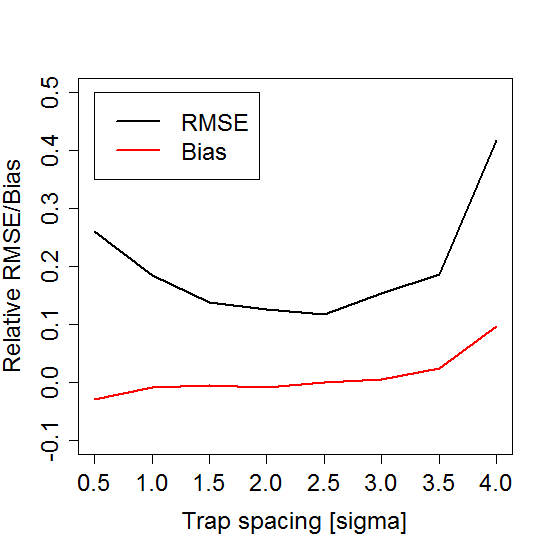
\includegraphics[width=3in]{Ch10-Design/figs/RMSE2.png}
\caption{Relative bias and RRMSE of estimates of $N$ from an SCR model for a range of trap spacing scenarios.}
\label{design.fig.rmse}
\end{figure}






\subsection{Black bears from Pictured Rocks National Lakeshore}

To see how trap array size influences parameter estimates from spatial
capture-recapture models in the real world, \citet{sollmann_etal:2012}
also looked at a black bear data set from Pictured Rocks National
Lakeshore, Michigan, collected using 123 hair snares distributed over
an area of 440 km$^2$ along the shore of Lake Superior in May-July
2005 \citep{belant_etal:2005}.  The SCR model for the bear data
included sex-specific
encounter rate parameters, and an occasion-specific baseline encounter
rate.
This was motivated by a) the lower average number of
detections for male bears, b) the decreasing number of detections
over time in the raw data, and c) the fact that male black bears are
known to move over larger areas than females (e.g.,
\citealp{gardner_etal:2010jwm, koehler_pierce:2003}).

To address the impact of a smaller trap array on the parameter
estimates, models fitted to the full data set were compared to
models fitted to data subsets.
The first subset retained only those 50\% of the traps
closest to the grid center. In the second, only the southern 20\% of
the traps were retained \ref{design.tab.bears}.

\begin{table}[ht]
  \centering
  \caption{Posterior summaries of SCR model parameters for black
    bears, modified from \citet{sollmann_etal:2012}.}
    \begin{tabular}{lrrrr}
%    \addlinespace
	\hline
          & Mean (SE) & Mode  & 2.5\% & 97.5\% \\ \hline
    {\bf Full data set} &       &       &       &       \\
    {\it D } & 10.556 (1.076) & 10.448 & 8.594 & 12.792 \\
    $\sigma^*$ (males) & 7.451 (0.496) & 7.323 & 6.579 & 8.495 \\
    $\sigma^*$ (females) & 2.935 (0.143) & 2.939 & 2.671 & 3.226 \\
    {\bf 50\% of traps} &       &       &       &      \\
    {\it D } & 12.648 (1.838) & 12.205 & 9.307 & 16.713 \\
    $\sigma^*$ (males)  & 5.354 (0.511) & 5.248 & 4.472 & 6.473  \\
    $\sigma^*$ (females) & 3.318  (0.277) & 3.262 & 2.841 & 3.910 \\
    {\bf 20\% of traps} &       &       &       &        \\
    {\it D } & 6.752 (1.611) & 5.953 & 4.000 & 10.218  \\
    $\sigma^*$(males)  & 9.881 (3.572) & 7.566 & 5.121 & 18.447 \\
    $\sigma^*$ (females)  & 2.686 (0.391) & 2.657 & 2.121 & 3.404  \\
    \hline
    \end{tabular}
  \label{design.tab.bears}
\end{table}

Reducing the area of the trap array by 50\% created a grid polygon of
144 km$^2$, which was smaller than an estimated male black bear home
range and only 50\% larger than a female black bear home range --
approximately 260 km$^2$ and 100 km$^2$, respectively, when converting
estimates of $\sigma^*$ to home range size. Table
\ref{design.tab.bears} shows that this did not greatly influence model
results, compared to the full data set.


Removing 80\% of the traps and thereby
reducing the area of the trap array to 64 km$^2$ -- well below the
average black bear home range -- had a great effect on sample size
(only 25 of the original 83 individuals sampled) and parameter
estimates. Particularly, male black bear movement was overestimated
and imprecise. The combination of the low baseline trap encounter rate
of males and the considerable reduction in sample size led to a low
level of information on male movement: 5 of the 12 males were captured
at one trap only. Although they moved over smaller areas, owing to
their higher trap encounter rate, females were, on average, captured at
more traps (3.4 traps per individual compared to 2.6 for males) so
that their movement estimate remained relatively
accurate. Overestimated male movements and female trap encounter rates
resulted in an underestimate of density of almost 40\%. This effect
is contrary to what we would expect to see in non-spatial CR models,
where a trapping grid that is small relative to animal movement
leads to underestimated movement (MMDM) and
overestimated density \citep{bondrup-nielsen:1983, dillon_kelly:2007,
  maffei_noss:2008}. While this example again demonstrates the ability
of SCR models to deal with a range of trapping grid sizes, it also
clearly shows that your study design needs to consider the amount of
data you can expect to collect. As an alternative to simulation studies, \citet{efford_etal:2009ecol} provide a mathematical procedure to
determine the expected number of individuals captured and recaptures
for a given detector array and set of model parameters.


\section{Sampling Over Large Areas}
\label{sec.design.large}

Trap spacing is an essential aspect of design of SCR studies. However,
it is only the most important aspect if one can uniformly cover a
study area with traps.   In many practical situations, where the study
area is large relative to effort that can be expended, one has to
consider other strategies which deviate from a strict focus on trap
spacing. There are two general strategies that have been suggested for
sampling large areas
which we think are useful in practice, either by themselves or
combined: Sampling based on {\it clusters} of traps and sampling based
on {\it rotating} groups of traps over the landscape.

\citet{karanth_nichols:2002} describe 3 strategies for  moving traps to
achieve coverage of a larger study area, geared toward traditional
capture-recapture analysis. Suppose that sampling the entire area of interest
requires sampling $G$ sites,
then the 3 strategies are:
\begin{itemize}
\item[   {\bf (1)}] For every day/sampling occasion, randomly choose
$x$ out of your $G$ sites, where $x$ is the number of trapping devices
you have at hand. Obviously, this requires that it be relatively easy
to move traps around.
\item[   {\bf (2)}] Move blocks of traps
that are close to each other in space daily. For example, if you
divide your total study area into 4 blocks, sample block 1 for a day,
then move traps to block 2 for a day, and so forth, and repeat until
each block has been sampled for a sufficient amount of time.
\item[   {\bf (3)}] If moving blocks of traps daily is too
challenging logistically, then you can sample each block for a
certain number of days/occasions before moving cameras to the next
block. In this fashion, you only need to move traps to each block
once.
\end{itemize}

In traditional CR we collapse data across traps and assume all
individuals in the study area have some probability $>0$ of being
detected. For our data that means that, under scenario (2) the first
occasion is defined as the time it takes to sample all 4 blocks once,
the second occasion consists of the second round of sampling all
blocks, etc. Under scenario (3), we have to combine data from day 1 in
each of the blocks to form occasion 1, data from day 2 in each of the
blocks forms occasion 2, and so on. Especially scenario 3 makes
modeling time-dependent detection difficult, since occasion 1 does no
longer refer to an actual day or continuous time interval.
We do not have that problem in SCR, where accounting for
 sampling effort at each trap is straight forward, as we first demonstrated
for the wolverine example in Sec. \ref{scr0.sec.wolverine}. Because we
are dealing with detection at the trap level, even for design (3) in a
spatial framework, we can still look at variation in detection over
time. As such, we don't think that one of the above designs is
superior for SCR models than the other, but rather, all of them may
produce adequate SCR data, as long as overall sample size requirements
are met.

\citet{efford_fewster:2012} looked at the performance of different
spatial study designs for abundance estimation from traditional and
spatial capture-recapture models, including a clustered design, where
groups of detectors are spaced throughout the larger region of
interest. They found that in a spatial framework this design performed
well, although there were indications of a slight positive bias in
estimates of $N$. Such a clustered design enables researchers to
increase area coverage without having to increase the number of
traps. \citet{efford_fewster:2012} note that distribution of clusters
has to be spatially representative -- for example, systematic with a
random origin.  The issue of spatially representative designs is not
limited to SCR and an extensive treatment of the topic can be found in
the distance sampling literature \citep{buckland_etal:2001}. Further,
the authors stress that, if distances among clusters are large and
individuals are unlikely to show up in several clusters, then the
method relies on spatial recaptures {\it within} clusters, meaning
that spacing of detectors within clusters has to be appropriate to the
movements of the species under study.  A clustered type of design is
also suggested by \citet{efford_etal:2009ecol} for acoustic detectors
(see Chapt. \ref{poisson-mn.sec.acoustic}) with small groups of such
detectors (e.g., $2 \times 2$) being distributed in a probabilistic
fashion across the region of interest.

In practice, employing both of these strategies -- clustering and
rotating traps -- might be necessary or advantageous.
\citet{sun:2013} used a simulation study to investigate different trap
arrangements (Fig. \ref{design.fig.sun}) for a black bear study based
on hair snares distributed over a 2625-km$^2$ study area. She
simulated detection data of bears for 3 trap arrangements including a
regular (uniform) coverage of traps, clusters of 4 traps each
with a gap between clusters, and a design in which the clusters were moved mid-way through the study to fill the gap (a
sequential or ``rotating'' design).  She found that the precision and
accuracy of estimates of $N$ generally decreased when changing from a
uniform to a clustered to a rotating design, although the loss of
efficiency was relatively small when using the clustered design. The
result seems to support that cluster designs can be effective with
relatively little loss of efficiency.

Further research on optimal detector configurations, especially for
large scale studies, is called for \citep{efford_fewster:2012}. More
generally, work on formalizing and generalizing these ideas of spatial
study design is needed.  We believe the model-based spatial design
approach that we introduce below is one possible way to do that.

\begin{figure}[ht]
\centering
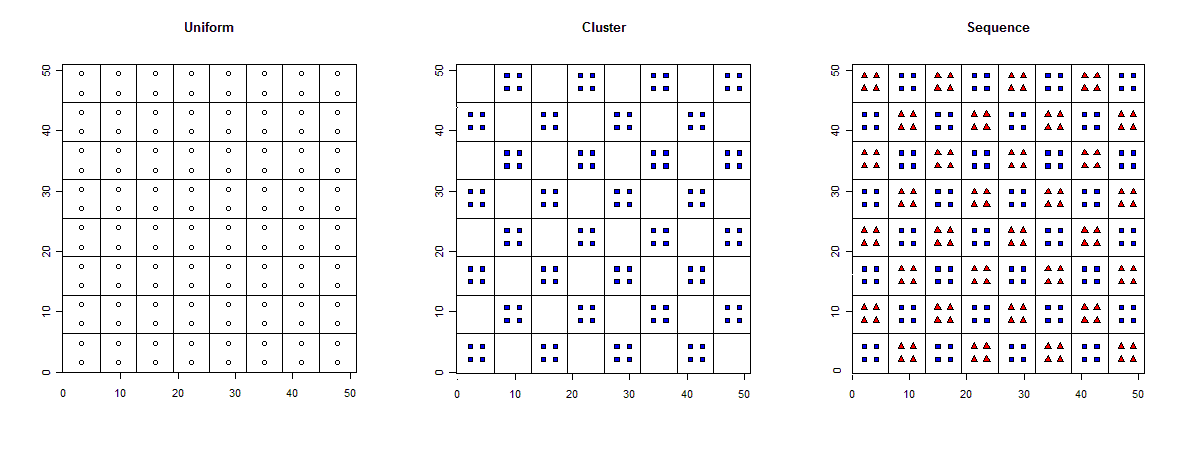
\includegraphics[width=5in,height=1.94in]{Ch10-Design/figs/catsun_designs.png}
\caption{Three designs evaluated by \citet{sun:2013}. The left panel
  shows uniform coverage of the area with traps (hair snares) equally
  spaced and static for the duration of the period. The central panel
  shows clusters of 4 traps in close proximity, with larger gaps
  between clusters. The right panel shows a design in which all grid
  cells are sampled by the cluster of 4 traps, but in a sequential (in
  time) manner.}
\label{design.fig.sun}
\end{figure}




\section{Model-Based Spatial Design}

A point we have stressed in previous chapters is that SCR models are
basically glorified versions of generalized linear models (GLMs) with
a random effect that represents a latent spatial attribute of
individuals, the activity center or home
range center.  This formulation makes analysis of the models readily
accessible in freely available software and also allows us to adapt
and use concepts from this broad class of models to solve problems in
spatial capture recapture. In particular, we can exploit
well-established model-based design concepts
\citep{kiefer:1959,
box_draper:1959,
box_draper:1987,
fedorov:1972,
sacks_etal:1989,
hardin_sloane:1993,
fedorov_hackl:1997}
to develop a framework for designing
spatial trapping arrays for capture-recapture studies.
\citet{muller:2007} provides a recent monograph level treatment of the subject
that is very accessible.

In the following sections, we adapt these classical methods for
constructing optimal designs to obtain the configuration of traps (or
sampling devices) in some region (the design space, ${\cal X}$),
that
minimizes some appropriate objective function based on 
the variance of model parameters,
${\bm \alpha}$, or $N$, for a prescribed
state-space. 
We show that this criterion -- based on the variance of
an estimator of $N$ -- represents a formal compromise between
minimizing the variance of the MLEs of the detection model parameters
and obtaining a high expected probability of capture.
Intuitively, if our only objective was to minimize the variance of
parameter estimates than all of our traps should be in one or a small
number of clusters where we can recapture a small number of
individuals many times each. Conversely, if our objective was only to
maximize the expected probability of encounter then the array should
be highly uniform so as to maximize the number of individuals being
exposed to capture.  



\subsection{Statement of the design problem}

Let ${\cal X}$, the {\it design space}, denote some region within
which sampling could occur and let ${\bf X} = {\bf x}_{1},\ldots, {\bf
  x}_{J}$ denote the {\it design}, the set of sample locations (e.g.,
of camera traps), normally we just call these ``traps.''  The design
space ${\cal X}$ must be prescribed (a priori).  Operationally, we
could equate ${\cal X}$ to the study area itself (which is of
management interest) but, in practical cases, there will generally be parts of
the study area that we cannot sample. Those areas need to be excluded
from ${\cal X}$.  While ${\cal X}$ may be continuous, in practice it
will be sufficient to represent ${\cal X}$ by a discrete collection of
points which is what we do here.  
This is especially convenient when
the geometry of ${\cal X}$ is complicated and irregular, which would
be the case in most practical applications.  The technical problem
addressed subsequently is how do we choose the locations ${\bf X}$ in
a manner that produces the ``optimal'' (lowest variance) for
estimating population size or density, or some other quantity of
interest. 

As usual, we regard the population of $N$ individual ``activity
centers'' as the outcome of a point process
 distributed uniformly
over the state-space ${\cal S}$.  The relevance and importance of
${\cal S}$ has been established repeatedly in this book, as it
defines a population of individuals (i.e., activity
centers) and, in practice, it is not usually the same as ${\cal X}$
due to the fact that animals move freely over the landscape and the
location of traps is typically restricted by policies, ownership, logistics and
other considerations.  
The objective we pursue here is: Given (1)
${\cal X}$, (2) a number of design points, $J$; (3) the state-space
${\cal S}$,
(4) an SCR model, and (5) a design criterion $Q({\bf X})$, we want
to choose {\it which} $J$ design points we should select in order to
obtain the {\it optimal} design under the chosen model, where the
optimality is with respect to $Q({\bf X})$.

What types of functions make reasonable objective functions, $Q({\bf
  X})$?  We will describe some possible choices for $Q({\bf X})$
below, but it makes sense that they should relate to the variance of
estimators of one or more parameters of the SCR model.

We motivate the basic ideas of model-based design with a simple model
that proves to be an effective caricature of the SCR model that we'll
use shortly. Suppose ${\bf s}$ is the activity center of a single
individual, and ${\bf s}$ is known with certainty.  Then, for an array
of traps ${\bf X}$ we measure a response variable, lets say the
strength of an
acoustic signal,
 that has a normal
distribution.
So we have this response variable that has a normal
linear model of the form:
\[
{\bf y} = {\bf M}({\bf X},{\bf s})'{\bm \alpha} + \mbox{error}
\]
In our notation here, ${\bf M}({\bf X},{\bf s})$ is some design matrix
where, in the context of SCR models, it has 2 columns (for the basic
model): A column of 1's, and then a column of distance from each trap
${\bf x}_{j}$ to the activity center ${\bf s}$. The design matrix is
therefore, for a single individual, a matrix of dimension $J \times
2$.

The inference objective here is to estimate the parameters ${\bm
  \alpha}$.  The variance-covariance matrix of $\hat{\bm \alpha}$ is,
suppressing the dependence on ${\bf X}$ for notational convenience,
\[
 \mbox{Var}( {\bm \alpha},{\bf X}) = ({\bf M}({\bf s})'{\bf M}({\bf s}))^{-1}
\]
Note that the design points ${\bf x}_{j}$ appear explicitly (in the
2nd column of {\bf M}).  In considering design for estimation in such
models it is natural to choose design points, corresponding to values
of ${\bf x}$, such that the variance of $\hat{\bm \alpha}$ is
minimized.  Of course, ${\bm \alpha}$ is a vector, and so the
``variance'' is a matrix (at least $2 \times 2$) so we have to work
with suitable scalar summaries of that matrix, such as the trace (sum
of the diagonals) or a function of the determinant, etc.. 

For a population of $N$ individuals, if we know {\it all} $N$ values
of ${\bf s}$, the design matrix ${\bf M}$ has the same basic structure
but with $N$ versions 
stacked-up on top of one another, producing a larger $N*J \times 2$
design matrix.  The 2nd column of that matrix contains the information
about trap locations (the 1st column is still just a column of 1s). 
Therefore, 
 we could easily find the design ${\bf X}$ that
optimizes some function of the variance-covariance matrix of the model
parameters.

All of this is fine and good if we happen to know the activity
centers for each individual. However, this is not a realistic
formulation. When ${\bf s}$ is unknown, it might make sense to consider
minimizing the expected (spatially averaged) variance:
\[
  E_{{\bf s}}\left\{ \mbox{Var}({\bm \alpha},{\bf X}) \right\} = \sum_{s \in
    {\cal S}}  ({\bf M}'({\bf s}){\bf M}({\bf s}))^{-1}.
\]
However, this is not the expected variance based on sampling a population
of $N$ individuals, just for a single individual having unknown ${\bf
  s}$. Because of the matrix inverse in this expression, it is not
sufficient to use a variance criterion that weighs this variance by
$N$.  As an alternative, we can
maximize the expected {\it information}, the inverse of the
variance-covariance matrix, which is probably more
appealing from an analytic point of view.  The information matrix for
the data based on a single individual, with known ${\bf s}$, is:
${\cal I}({\bm \alpha},{\bf X}) =
 ({\bf M}'({\bf s}){\bf M}({\bf s}))$.
For a population of $N$ individuals, let ${\bf M}_{i}$ be the design
matrix for the individual with
activity center ${\bf s}_{i}$. Then, the total information for all $N$
individuals is:
\[
 {\cal I}({\bm \alpha},{\bf X}) = 
 \sum_{i=1}^{N}  ({\bf M}_{i}'({\bf s}_{i}){\bf M}_{i}({\bf s}_{i}))
\]
The information matrix depends on the design ${\bf X}$ through the $N$
individual matrices ${\bf M}_{1},\ldots,{\bf M}_{N})$.
Now, because we don't know ${\bf s}_{i}$ we can compute the integrated
information, over all possible values of ${\bf s}_{i}$, and for {\it
  each} ${\bf s}_{i}$, which is an $N$-fold summation:
\[
E_{ {\bf s}_{1}, \ldots, {\bf s}_{N}}
 {\cal I}({\bm \alpha},{\bf X}) = 
 \sum_{i=1}^{N}  \sum_{s \in {\cal S}} ({\bf M}_{i}'({\bf s}_{i}){\bf M}_{i}({\bf s}_{i}))
\]
which is just $N$ copies of
the integrated (spatially averaged) information:
\[
E_{ {\bf s}_{1}, \ldots, {\bf s}_{N}}
 {\cal I}({\bm \alpha},{\bf X})
=  N \sum_{s \in {\cal S}} ({\bf M}_{i}'({\bf s}_{i}){\bf M}_{i}({\bf s}_{i})).
\]

It therefore seems sensible to base design of SCR studies on some
criterion that is a function of this expected information
matrix. E.g., find the design that maximizes the diagonals, or the
determinant, or minimizes the trace of the {\it inverse} (the
variance-covariance matrix based on $N$ individuals).  
This can be done for any number of design points ${\bf
  x}_{1},\ldots, {\bf x}_{J}$ using standard exchange algorithms
\citep[see][Chapt. 3]{muller:2007} and we discuss this below in
Sec. \ref{design.sec.exchange}.
However, our SCR models are not normal linear models but, rather, more
like Poisson or binomial GLMs. We see in the next section that we can
adapt these ideas for such models.


\subsection{Model-based Design for SCR}

Following our development of the normal linear model above, suppose
for the moment that we know ${\bf s}$ for a single individual.  In
this case, its vector of counts of encounter in each trap ${\bf y}$
are either binomial or Poisson counts, and the linear predictor has
this form:
\begin{equation}
g( \mathbb{E}({\bf y})  ) =  \alpha_0  + \alpha_1 ||{\bf x}-{\bf s}||^2.
\label{eq.linearpredictor}
\end{equation}
for the Gaussian encounter probability model, or any other model could
be used. In vector form, we write this as:
\[
g( \mathbb{E}({\bf y})  ) =  {\bf M}'{\bm \alpha}
\]
where ${\bf M}$ is the $J \times 2$ design matrix where the 2nd column
contains the squared pairwise distances between each individual $i$
and trap $j$, and thus it depends on both ${\bf X}$ and ${\bf s}$.

The asymptotic formula for $\mbox{Var}( {\bm \alpha})$ can be cooked
up for any type of GLM. As an example (we use this below), for the
Poisson GLM, the asymptotic variance-covariance matrix of $\hat{\bm
  \alpha}$, considering a single individual having location ${\bf s}$,
is\footnote{ This is basic GLM theory that derives from the fact that
  the Poisson is a member of the natural exponential family of
  distributions, e.g., see \citet{mccullagh_nelder:1989} or
  \citet{agresti:2002}.}
\begin{equation}
  \mbox{Var}(\hat{\bm \alpha}|{\bf X},{\bf s})
=  ({\bf M}({\bf s})' {\bf D}({\bm \alpha},{\bf s}){\bf M}({\bf s}))^{-1}.
\label{eq.varalpha}
\end{equation}
This is a function of the design ${\bf X}$ as well as ${\bf s}$ both
of which are balled-up in the regression design matrix ${\bf M}$, and
the matrix ${\bf D}$ which is a diagonal matrix having elements
$\mbox{Var}( y_{j}|{\bf s}) = \exp({\bf m}'{\bm \alpha})$ for $y_{j} =$
the frequency of encounter in trap $j$ and where ${\bf m}'$ is the j$^{th}$ row
of ${\bf M}({\bf s})$. 
We can compute the expected
information under the Poisson model with known $N$ using this modified
formulation.  These ideas are meant to motivate technical concepts
related to model-based design, where we know $N$, and therefore have a
convenient variance or information expression to work with. However,
in all real capture-recapture applications we won't know $N$, and so
we need to address that issue, which we do in the next section.



\subsection{An Optimal Design Criterion for SCR}

There are a number of appealing directions to pursue for deriving a
variance-based criterion upon which to devise designs for capture
recapture studies.  For one, we could formulate the objective function
based on the variance of the Huggins-Alho estimator (Sec. \ref{closed.sec.indcov}) of $N$.  
We find that these expressions depend on individual sample inclusion
probabilities (if ${\bf s}$ is close to traps, the individual has a
high probability of being encountered and {\it vice versa}), and hence
the specific trap locations, and parameters of the model.  These
variance expressions provide a natural design criterion. On the other
hand, we find that the calculus is a bit tedious at the present time.
%We might also consider the MLEs based on the marginal Poisson or
%Binomial likelihoods, and then we could possibly compute the
%variance-covariance matrix of the MLEs directly.  This merits further
%investigation.  
As an alternative, we
devise a variance criterion based on the conditional estimator of $N$
having the form
\[
  \tilde{N}  =  \frac{n}{\hat{\bar{p}}}
\]
where $\hat{\bar{p}}$ is the MLE of the marginal probability that an
individual appears in the sample of $n$ unique individuals, and it
depends on the MLE of the parameters of the encounter probability
model, $\hat{\bm \alpha}$.  We elaborate on the precise form of
$\bar{p}$ and the variance of its MLE below.  The variance of this
estimator is:
\[
\mbox{Var}(\frac{n}{\hat{\bar{p}}}) = n^2 * \mbox{Var}(
\frac{1}{\hat{\bar{p}}} )
\]
An important thing to note is that this estimator, and its variance, 
are  {\it conditional}
on the sample size of individuals, $n$. We never set out, in capture-recapture, to obtain a sample of
$n$ individuals ($n$ is always a stochastic outcome) and so we need to 
``uncondition'' on $n$.
Fortunately, this is a simple proposition using standard rules of
expectation and variance, which produce the following expression:
\begin{equation}
 \mbox{Var}(\tilde{N}(\bm \alpha) ) =
  N \bar{p} \left\{ (1-\bar{p}) + N \bar{p} \right\}
\left( \frac{ \mbox{Var}( \hat{\bar{p}}) } { \bar{p}^{4} } \right)
\label{design.eq.theQ}
\end{equation}
The key thing to note about this as a criterion:
 (1) It depends on $\bar{p}$, the marginal probability of
 encounter. Clearly the variance decreases as $\bar{p}$ increases. In
 general, the form of $\bar{p}$ depends on the SCR model being used. We
 will provide an example below. Obviously, $\bar{p}$ will depend on
 the parameter values ${\bm \alpha}$. 
 (2) The criterion depends on $\mbox{Var}(\hat{\bar{p}})$. So, designs
 that estimate $\bar{p}$ well should be preferred.  This will also
 depend on the parameters ${\bm \alpha}$ and {\it also} the variance
 of the MLE, $\hat{\bm \alpha}$. 
 Based on these considerations, 
we suggest a number of appealing criteria for constructing spatial
designs for capture-recapture studies.
For convenience we label them $Q_{1}$ - $Q_{4}$:
\begin{itemize}
\item[(1)] $Q_{1} = \mbox{Trace}({\bf V}_{\hat{\bm \alpha}})$ where ${\bf
    V}_{\hat{\bm \alpha}}$ is the variance-covariance matrix of the
  MLE of ${\bm \alpha}$. Designs which minimize this criterion
  are those which are good for estimating the parameters of the
  encounter probability model. 
\item[(2)] $Q_{2}$ is the variance expression in
  Eq. \ref{design.eq.theQ}. Using this criterion, we should prefer designs that minimize
  the variance for estimating $N$.
\item[(3)] $Q_{3} = 1-\bar{p}$. Designs which minimize this criterion
  are those which maximize the average capture probability. These
  should maximize $n$.
\item[(4)] $Q_{4} = \mbox{Var}(\hat{\bar{p}})$. We should prefer
  designs which provide good estimates of $\bar{p}$. 
\end{itemize}
To make use of any of these criteria in a particular design problem, we need
to decide on values of $N$, and the model parameters for computing
$\bar{p}$, and then think about optimizing the criterion over all
possible designs (see below).



\subsection{Too much math for a Sunday afternoon}

Here we discuss calculation $\bar{p}$ and variance expressions
required to compute the design criteria above. 

\subsubsection{Characterizing $\bar{p}$}

In SCR models, an individual with activity center ${\bf
  s}_{i}$ is captured if it is captured in {\it any} trap and
therefore, under the Bernoulli (passive detector) observation model,
\[
 \bar{p}({\bf s}_{i}, {\bf X}) = 1 - \prod_{j=1}^{J} (1- p_{ij}({\bf
   x}_{j}, {\bf s}_{i}))
\]
where $p_{ij}$ here is the Gaussian (or other) encounter probability
model that depends on distance between traps and activity centers,
say $d_{ij}$ for the distance between 
individual activity center ${\bf s}_{i}$ and trap ${\bf x}_{j}$.
Under the Poisson observation model, with a Gaussian hazard model:
\[
 \bar{p}({\bf s}_{i},{\bf X}) = 1 -  \exp(-\lambda_{0} \sum_{j}
 \exp(\alpha_{1}* d({\bf x}_{j}, {\bf s}_{i})^2 ))
\]
where here we emphasized that this is conditional on ${\bf s}_{i}$ and
also the design -- the trap locations ${\bf x}_{j}$.  The {\it
  marginal} probability of encounter, averaging over all possible
locations of ${\bf s}$ is:
\begin{equation}
 \bar{p}({\bf X}) = 1 - \int_{\bf s}    \bar{p}({\bf s}_{i},{\bf X})    d{\bf s}.
\label{design.eq.pbar}
\end{equation}
It is important to note that this can be calculated directly {\it
  given} the design ${\bf X}$, and parameters of the model. This is
handy because we see that it is used in the variance formulae given
subsequently and therefore it is used directly in evaluating any of
the criteria described above.


\subsubsection{Characterizing $\mbox{Var}(\hat{\bar{p}})$}

Developing an expression for $\mbox{Var}(\hat{\bar{p}})$ depends on
the observation model. 
We work here with the Poisson observation model, and we do that
because the technical argument that follows is somewhat easier for
that case compared to the Bernoulli model for passive detection
devices (but see
\citet{huggins:1989} and \citet{alho:1990} for additional context). 
We first express the integral in Eq.
\ref{design.eq.pbar} as a summation over a fine mesh of points so
that:
\[
 \bar{p}({\bf X}) = \sum_{{\bf s}} 1 - \bar{p}({\bf s}_{i},{\bf X})
\]
which under the Poisson observation model is, in a simplified notation:
\[
 \bar{p}({\bf X}) = \sum_{{\bf s}} \left\{
1 -  \exp(- \sum_{j}
 \exp(\alpha_{0} + \alpha_{1}  d({\bf x}_{j}, {\bf s})^2))
\right\}
\]
The MLE of $\bar{p}({\bf X})$ has us plug in the MLE of the parameters
of the model, in this case $\hat{\lambda}_{0} = \exp(
\hat{\alpha}_{0})$ and $\hat{\alpha}_{1}$. 
To compute the variance of the MLE of $\bar{p}$, we note that the
variance operator can move inside the summation over ${\bf s}$, and
the subtraction from 1 doesn't count anything, so we have
\[
\mbox{Var}( \hat{\bar{p}}({\bf X}) ) = \sum_{{\bf s}} \mbox{Var}
\left( \exp(- \sum_{j} \exp(\hat{\alpha}_{0} + \hat{\alpha}_{1} d({\bf
    x}_{j}, {\bf s})^2)) \right)
\]
A few applications of the delta approximation and some arm-waving yields 
the following expression for the variance of
$\hat{\bar{p}}$:
\[
\mbox{Var}( \hat{\bar{p}}({\bf X}) )  =
\sum_{{\bf s}} \left( \exp( - \hat{\lambda}_{\bf s} )  \right)
\left(    \sum_{j}  \hat{\lambda}({\bf x}_{j},{\bf s})^{2} (
 \mbox{Var}( \hat{\alpha}_{0}) +
  d({\bf x}_{j}, {\bf    s})^4
\mbox{Var}( \hat{\alpha}_{1})  )
  \right)
\]
where $\lambda({\bf x},{\bf s}) = \exp( \alpha_{0} + \alpha_{1} d({\bf
  x},{\bf s})^{2})$ and $\lambda_{\bf s} = \sum_{j=1}^{J} \lambda({\bf
  x}_{j},{\bf s})$.


\subsubsection{Characterizing $\mbox{Var}( \hat{\bm \alpha})$ }

The big picture is this: For a given design ${\bf X}$, we can compute
$\mbox{Var}(\hat{\bar{p}}({\bf X}))$ -- this is just a calculation
involving sums over all points in the state-space and design points
-- provided we know the variance of the estimator of ${\bm \alpha}$,
$\mbox{Var}(\hat{\bm \alpha})$ and the parameters of the model.
However, it is not so easy to write down the analytic form of this
matrix.  Some calculus would have to be done on the conditional
likelihood (e.g., from \citet{borchers_efford:2008}) to figure out the
asymptotic form of this matrix.  For our purposes, we think it might
suffice\footnote{Warning: But we don't know. No warranty is implied.}
to a approximate the matrix, using the analogous result from a Poisson
or binomial GLM assuming that $N$ is known, since we have convenient
formulas for those (see Eq. \ref{eq.varalpha}).

The approximate variance given by Eq. \ref{eq.varalpha}
is conditional on the collection of activity centers, ${\bf
  s}_{1},\ldots,{\bf s}_{N}$. To resolve this, we take the approach
outlined previously to compute the {\it expected} information obtained
from a particular realization of $N$ individuals, and invert that
result. In particular, the total information for all $N$ individuals
is
\[
{\cal I}(N) =  {\bf M}_{1}' {\bf D}_{1} {\bf M}_{1} + \ldots +
{\bf M}_{N}{\bf D}_{N} {\bf M}_{N}
\]
We can compute
the expected information over {\it all} elements of the state-space,
which is just $N$ times the average information of a single
individual:
\[
\mathbb{E}( {\cal I}(N) ) = N  \sum_{{\bf s}}  {\bf M}({\bf s})'{\bf
  D}({\bf s}) {\bf M}({\bf s}).
\]


\subsubsection{Putting it all together}

For a single design, ${\bf X}$, we need
to compute this expected information quantity, invert it to get the
variance of $\hat{\bm \alpha}$, and then either use that variance
matrix in the calculation of criterion $Q_{1}$, or else evaluate some
other quantities along the way to computing the other criteria. 
We can compute $\bar{p}$ (which is $Q_{3}$) for a given design without
doing any variance calculations. 
If we use $\mbox{Var}(\hat{\bm \alpha})$ along with $\bar{p}$, we can
compute $\mbox{Var}(\hat{\bar{p}})$, which is $Q_{4}$. 
We can combine all of these things together and compute
$\mbox{Var}(\tilde{N})$ for a given ${\bf X}$. This gives us $Q_2$. 



\subsection{Optimization of the criterion}
\label{design.sec.exchange}


To compute spatial designs that optimize a given criterion, we need to
come up with a ballpark guess of the model parameters so that the
criterion can be evaluated for any design. i.e., what are the values of
${\bm \alpha}$ and $N$ we expect in our study?  If we do that, and
specify the state-space ${\cal S}$ then, we can, in theory, optimize
the variance criterion over all possible configurations of $J$ traps.
In formulating the optimization problem note that we have $J$ sample
locations corresponding to rows of ${\bf X}$.  The problem is
therefore a $2J$ dimensional optimization problem which, for $J$
small, could be solved using standard numerical optimization
algorithms as exist in almost every statistical computation
environment.  However, $J$ will almost always be large enough so as to
preclude effective use of such algorithms. This is a common problem in
experimental design, and spatial sampling in general, for which
sequential exchange or swapping algorithms have been fairly widely
adopted \citep[e.g.,][]{wynn:1970, fedorov:1972, mitchell:1974,
  meyer_nachtsheim:1995,nychka_etal:1997,royle_nychka:1998}.  The
basic idea is to pose the problem as a sequence of 1-dimensional
optimization problems in which the objective function is optimized
over 1 or several coordinates at a time.  In the present case, we
consider swapping out ${\bf x}_{j}$ for some point in ${\cal X}$ that
is nearby ${\bf x}_{j}$ (e.g., a 1st order neighbor). Beginning with
an initial design, chosen randomly or by some other method, the
objective function is evaluated for all possible swaps (at most 4 in
the case of 1st order neighbors) and whichever point yields the
biggest improvement is swapped for the current value.  The algorithm
is iterated over all $J$ design points and this continues until
convergence is achieved. Such algorithms may yield local optima and
optimization for a number of random initial designs can yield
incremental improvements. We implemented such a swapping algorithm in
{\bf R}, and it is available as a function in the \mbox{\tt scrbook}
package with the function \mbox{\tt SCRdesign}.  The algorithm
operates on a discrete representation of ${\cal S}$ (an arbitrary
matrix of coordinates).  For each point in the design, ${\bf X}$, only
the nearest neighbors (the number is specified by the user) are
considered for swapping into the design during each iteration.  For
example, to compute \mbox{\tt ndesigns = } 10 putative optimal designs
(each based on a random start) of size $J=11$, we execute the function
as follows:
\begin{verbatim}
> des<-SCRdesign(S,X,ntraps=11,ndesigns=10,nn=15,sigma=1)
\end{verbatim}
Where the state-space \mbox{\tt S}, the candidate set \mbox{\tt X} are
provided as matrices, \mbox{\tt nn} is the number of nearest neighbors
to inspect for each design point change, and \mbox{\tt sigma} is the scale
parameter of, in this case, a Gaussian hazard model. See the help file
\mbox{\tt SCRdesign} for examples and analysis of the output. 


While swapping algorithms are convenient to implement, and efficient
at reducing the criterion in very high dimensional problems, they do
not always yield the global optimum.  In practice, as in the examples
below, it is advisable to apply the algorithm to a large number of
random starting designs.  Our experience is that essentially
meaningless improvements are realized after searching through a few
dozen random starts.

The design criteria we developed above bear a striking resemblance
to design criteria used to construct so-called space-filling designs
\citep{nychka_etal:1997}. Such criteria are based on inter-point
distances, and space-filling designs seek to optimize some function of
distance alone, instead of a variance-based objective function. The
benefit of this approach is that one doesn't have to specify the model
to produce a design, and space-filling designs have been shown to
provide reasonable approximations to designs based on variance
criteria under flexible
statistical models \citep{nychka_etal:1997}. 
This similarity suggests that perhaps
certain distance-based design criteria might be suitable for SCR
models. A version of a swapping algorithm used to
optimize a space-filling criterion is implemented in the {\bf R}
package {\bf fields}.


\subsection{Illustration}

Because the algorithm operates on a discrete version of ${\cal S}$,
it is trivial to apply to situations in which the
state-space is arbitrary in extent and geometry. However, we consider
a simplified situation here in order to illustrate the calculation of
optimal designs and how they look for an idealized situation.

Consider designing a camera trapping study for a square state-space on
$[9,21] \times [9, 21]$ and with ${\cal X}$ being the smaller square
$[10,20] \times [10,20]$.  For this illustration we assumed
$\alpha_{0} = \log(\lambda_{0}) = -1.7$ and $\sigma=\sqrt{2}$ so that
$\alpha_{1} = 1/(2\sigma^{2}) = 1/4$.

Designs of size 11 and 21 were computed using 10 random starting
designs.  We found the optimal design using each of the 4 criteria we
described above. To refresh your memory $Q_{1}$ is the trace of the
variance-covariance matrix of $\hat{\bm \alpha}$, $Q_{2}$ is the
variance of $\tilde{N}$, $Q_{3}$ is $1-\bar{p}$ (so the design that
minimizes this criterion obtains the highest possible $\bar{p}$), and
$Q_{4}$ is the variance of $\hat{\bar{p}}$.  The putative optimal
designs (henceforth ``best'') are shown in
Fig. \ref{design.fig.designs}. There are a few points of some interest
here.


The designs are not completely regular but obviously have a systematic
look to them. For the $J=11$ designs, the $Q_{1}$ design is slightly
more compact, with an average closest neighbor distance of $2.59$
units vs $3.03$ units for the $Q_{3}$ design. The two designs are
qualitatively similar, providing roughly uniform coverage of the
design space ${\cal X}$.  Conversely, the other two criteria produce
designs that are highly clustered.  Criterion $Q_{2}$ which is optimal
for $\tilde{N}$, produces 2
clusters of traps, 7 traps in one and 4 traps in the other. Finally,
designs which are optimal for the criterion $Q_{4}$, the variance of
estimating $\bar{p}$, produce a single cluster of traps that is
roughly centrally located in the design space. This makes sense,
because the very dense cluster of traps provides a large number of
recaptures near the origin $d=0$, which, intuitively, provides the most information
about estimating parameter of the encounter probability model. 
 For the $J=21$ designs, we have an average closest neighbor
distance of $1.87$ for $Q_{1}$ and $2.19$ for $Q_{3}$ but,
qualitatively, the structure of the designs is similar to $J=11$. The
best design for estimating $N$ (the criterion $Q_{2}$) produces 2
clusters, but just with more traps. While these illustrations
  make sense to us, we're not entirely convinced of the implication
  that 2 clusters of traps should be optimal with $J=21$ total
  traps. However, it is clear what is going on here is that the tight
  clusters are providing good information about estimating $\bar{p}$
  and, by spreading the two clusters out, the expected sample size,
  $n$, is maximized.

While the designs for $Q_{1}$ and $Q_{3}$ are not exactly uniform, they are very regular
looking which we should expect given the regularity of both ${\cal
  S}$ and ${\cal X}$ in this case.  One thing to note is that the trap
spacing varies depending on $J$ {\it even though} $\sigma$ is the
same, so optimal trap spacing should not be viewed as a static thing
depending only on the model.  Because the designs are not exactly
regular, the average closest neighbor distance is not exactly the same
as the trap spacing of a regular grid design. 



\begin{figure}[ht]
\centering
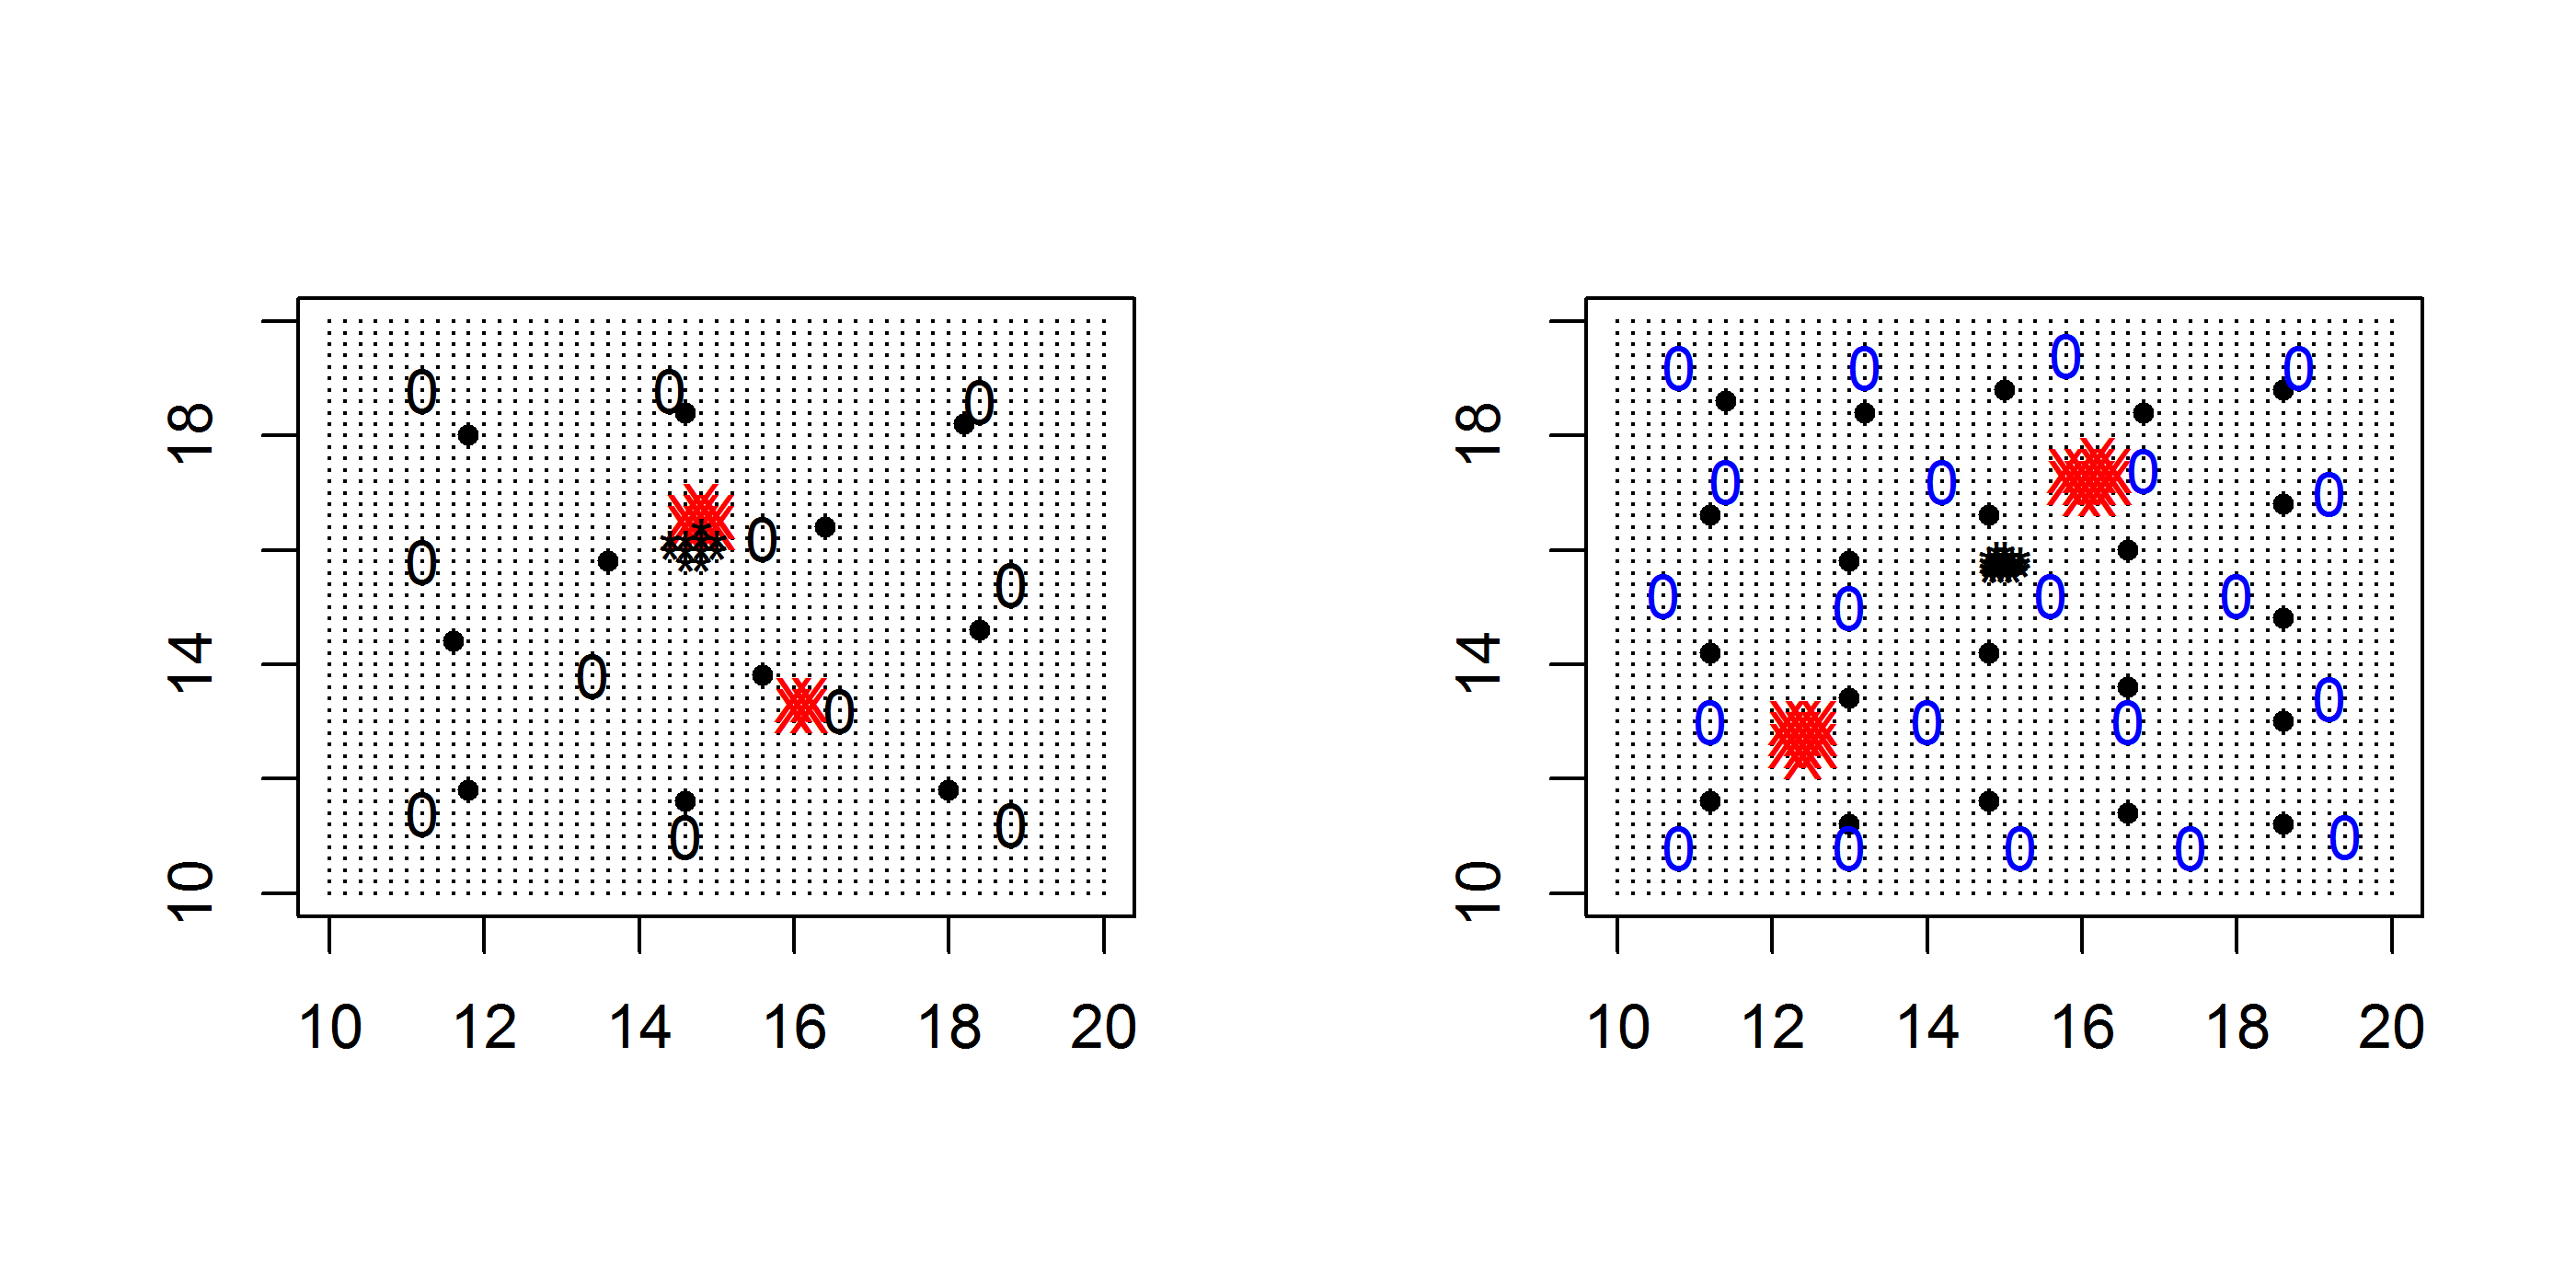
\includegraphics[width=4.8in]{Ch10-Design/figs/designs.png}
\caption{Best designs for each of 4 design criteria, produced using
  the exchange algorithm with 15 nearest-neighbors and based on 10
  random starting designs. The left panel shows the best $J=11$ point
  designs, and the right panel shows the best $J=21$ point
  designs. The solid black dots correspond to the best design for
  $Q_{1}$, $0$ marks the design for $Q_{3}$, ``X'' for $Q_{2}$ and the
  tightly clustered ``*'' corresponds to $Q_{4}$. 
}
\label{design.fig.designs}
\end{figure}


\subsection{Density covariate models}

Many capture-recapture studies will involve one or more landscape or
habitat covariates that are thought to affect density, with the idea
of using the methods described in Chapt. \ref{chapt.state-space} for
modeling and inference.  We imagine that it should be possible to
extend the model-based framework described previously to accommodate
uncertainty due to having to estimate ${\bm \beta}$, and this could be
included as a feature of the design criterion.

In this case, we can think
of the captures in a trap being Poisson random variables with mean
$\mu({\bf x},{\bf s})*D({\bf s})$ 
and we think the same arguments
as given above can be used to devise design criteria and optimize
them. However, in this case we might not only care about estimating
$N$ but also (or instead) inference about the parameters ${\bm
  \beta}$. Thus, we might choose designs that are good for $N$ or
perhaps only good for estimating ${\bm \beta}$ or perhaps both.
Intuitively, we think these two design objectives conflict with one
another to some extent.  Model-based approaches should favor areas of
higher density, but the design points need to realize variation in the
landscape covariates too.



\section{Temporal aspects of study design}

The spatial configuration of traps is one of the most important
aspects of sampling design for capture-recapture studies. Indeed, as
we discussed in the previous section, design under SCR models can be
thought of as being analogous to classical model-based spatial design,
and the concepts and methods from that field can be brought to bear on
the design of capture-recapture studies.
However, there are other aspects of sampling design that should be
considered in capture-recapture studies, including the frequency or
length of temporal samples. We discuss some of these issues here,
although without a detailed or formal analysis.

\subsection{Total sampling duration and population closure}

All the models we have discussed so far
are {\it closed population} SCR models, i.e., models that assume
that the population remains constant during our survey. Traditionally,
two different levels of closure have been considered in the
capture-recapture literature -- demographic and geographic closure
(see also Chapt. \ref{chapt.closed}). Demographic closure refers to
the absence of births and deaths, while geographic closure refers to
the absence of immigration and emigration during a study. In
traditional capture-recapture, the geographic closure assumption
prohibited (in theory, not in field praxis, of course) any movement
off the trapping grid.  \citet{kendall:1999} explored a range of
scenarios of closure violation, focusing on different kinds of
movement in and out of the study area, and found that several of these
scenarios caused biased abundance estimates from traditional
capture-recapture models.


As discussed in Chapt. \ref{chapt.scr0}, one main objective of SCR
models is to relax the geographic closure assumption -- the model
explicitly allows for movements of individuals about their activity
centers, which may have them off the trapping grid for parts of the
time, even if the activity center itself is on the grid. SCR models
do, however, assume no permanent emigration or immigration from the
state-space. The interpretation of demographic closure remains the
same in SCR models as it is in traditional CR models.

We have not explored effects of closure violation on SCR abundance and
density estimates. Conceptually, we expect estimates to be biased high
when births or immigrations happen during our study. For one, the
total number of individuals at the study site during the course of the
study would be higher than at any particular point in time and
correspond to a {\it cumulative} number of individuals in our study
area. Further, because some individuals are not available for
detection for the entire study (they only become available when they
are recruited) we would expect detection to be underestimated,
potentially leading to further positive bias in estimates of
abundance. Death or emigrations during a study do not inflate the
number of individuals actually on the study area, but as animals die
and become unavailable for detection, we can again imagine a negative
bias in baseline detection and, consequently, some positive bias in
$N$.

To avoid such bias in population estimates, closed population models
should typically be applied to short surveys, where short is relative
to the life history of the species under study. For example, for small
mammals, that might mean a few days, whereas for large, long-lived
species with a slow population turnover, several weeks or even a
couple of months can still be considered short. In practice, we have
no means of ever guaranteeing a closed population -- even if we sample
animals for a day, one of the individuals we record may be eaten by a
predator later that day, or a dispersing individual may arrive just as
we turn our backs. On the other hand, we are faced with the need to
collect sufficient data, which, especially for elusive species, pushes
us to sample over longer rather than shorter time periods. If we do
not have enough sampling devices to cover the entire area of interest
at once, rotating study designs (see sec. \ref{sec.design.large}) can require even
longer sampling to accumulate sufficient captures and recaptures. So
clearly, in temporal study design we have to strive for a compromise
between collecting enough data while still approximating a closed
population.  For some species we may be able to avoid seasons where
violation of demographic closure is particularly likely -- for example
migration seasons in migratory birds, or specific breeding seasons (or
collective suicide season in lemmings). But for many species such
biological seasons might be less clear cut. For example, in warm
climates tigers and other large cats can breed year round
\citep{nowak:1999}. As a consequence, guidelines as to what time frame
adequately approximates a closed population are generally vague and
arm-wavy. Unfortunately, we do not have much more to offer on the
subject of how to decide on the length of a study, other that to urge
you to think about the biology of your study species {\it before the
  study} and choose a time window that seems appropriate for that
purpose.

\subsection{Diagnosing and dealing with lack of closure}

Once a field study has been conducted, you may wonder whether the
collected data contain any evidence that the closure assumption has
been met or violated. Relatively few tests for population closure in
traditional capture-recapture have been developed, mostly due to the
fact that behavioral variation in detection is indistinguishable from
violation of demographic closure \citep{otis_etal:1978,
  white_etal:1982}. \citet{otis_etal:1978} developed a test for
population closure that can handle heterogeneity in detection
probability, but does not perform well in the presence of time or
behavioral variation in $p$. \citet{stanley_burnham:1999} developed a
closure test for model $M_t$ (time variation in detection), which
works well when there is permanent emigration and a large number of
individuals migrate. Both tests are implemented in the program {\bf
  CloseTest} \citet{stanley_richards:2005}.

There are no specific population closure tests for SCR models, for the
same reasons that violation of other model assumptions cannot
necessarily be distinguished from a lack of population closure. If you
are worried that closure might have been violated in your study, one
approach of dealing with this problem is to fit an open population
model. You can subdivide your study into several periods and
fit a spatial version of Pollock's robust design capture-recapture
model, which can estimate population size/density for each of these
periods
 (in this context also called primary periods) using models of
 demographic closure.
Alternatively, we may consider  fully dynamic models which
contain explicit parameters of survival and recruitment (Chapt. \ref{chapt.open}).
These models can be quite time consuming, and if you wanted a faster
check you could alternatively fit a spatial Cormack-Jolly-Seber model
that only estimates survival. The magnitude of the survival estimates
gives you some partial information about population closure in your
study -- if survival is close to 1 at least there is little evidence
of losses of individuals, either through permanent emigration or
death. These and other open population models are presented in detail
in Chapt. \ref{chapt.open}. Finally, if your data are too sparse to
fit a full-blown open population model, you can subdivide your study
into $t=1,2,...,T$ primary periods and estimate abundance separately
for each period's worth of data, possibly sharing the detection
parameters across periods, if you can safely assume they remain
constant. You can do that by either letting $N_t$ be independent from
each other, or by specifying an underlying distribution for all $N_t$
in a multi-session framework as described in Chapt. \ref{chapt.hscr}.

\section {Summary and Outlook}
\label{design.sec.outlook}

Design of capture-recapture studies in the context of {\it spatial}
models is an important problem, but solutions to this problem are
mostly {\it ad hoc} or incomplete at the present time. As a general
rule, we always recommend scenario analysis by Monte Carlo simulation
\citep{efford_fewster:2012, sollmann_etal:2012, sun:2013}.  This takes
a lot of time but it guarantees forward progress, or at least not
doing the dumbest from among several dumb things.  We discussed some
examples from the literature that assess trap spacing and
evaluate trap clustering and rotating coverage strategies for sampling
large areas.  The nice thing about simulation studies is that we can
simulate data for any complex situation we desire, even if we can't
fit the model effectively. Thus, we can always characterize worst-case
situations under pathological model misspecifications.

When designing a spatial capture-recapture study for a single species, trap
spacing and the size of the array can (and should) be tailored to the
spatial behavior of that species to ensure adequate data
collection. However, some trapping devices like camera traps may
collect data on more than one species and researchers may want to
analyze these data, too. Independent of the trapping device used,
study design will in most cases face a limit in terms of the number of
traps available or logistically manageable. As a consequence,
researchers need to find the best compromise between trap spacing and
the overall grid area.

Particularly for large mammal research, SCR models have much more
realistic requirements in terms of area coverage than non-spatial CR
models. In the latter, density estimates can be largely inflated with
small trapping grids relative to individual movement
\citep{maffei_noss:2008} -- covering at least 4 times the average home
range is recommended. Further, we need consistent coverage of the
entire study area, as all individuals in the population of interest
must have some probability $>0$ to be captured.

In contrast, SCR models work well in study areas on the scale of an
individual's home range (as long as sufficient data is collected)
\citep{sollmann_etal:2012, efford_etal:2011, marques_etal:2011}, and
they provide unbiased estimates for sampling designs that do not
expose all individuals in the sampled population to detectors, i.e.,
that have ``holes'' \citep{efford_fewster:2012}.  These results,
however, should not encourage researchers to design non-invasive trap
arrays based on minimum area requirements and with a minimum number of
detectors. Study design should still strive to expose as many
individuals as possible to sampling and obtain adequate data on
individual movement. Large amounts of data, both individuals and
recaptures, do not only improve precision of parameter estimates
\citep{sollmann_etal:2012, efford_etal:2004}, they also allow
including potentially important covariates (such as gender or time
effects in the black bear example -- see also
Chapt. \ref{chapt.covariates}) into SCR models to obtain density
estimates that reflect the actual state of the studied population.

Beyond the traditional grid-based sampling design, the flexibility of
SCR models allows for different spatial detector arrangements such as
linear (see \citet{efford_etal:2011} for an example), or dispersed
clusters of detectors. How well these different
designs perform, comparatively, remains to be explored.

The other general strategy for constructing spatial designs is a
formal model-based strategy in which we seek the configuration of
design points (trap locations) ${\bf x}_{1},\ldots, {\bf x}_{J}$ which
are optimal for some formal information-based objective function.
This is a standard approach in classical sampling and experimentation,
yet it has not gained widespread use in ecology. In our view,
model-based design under SCR models has great potential due to its
coherent formulation and flexibility.  On this topic, we have just
barely scratched the surface here, showing how to formulate a
criterion that is a function of the design, and then optimizing the
criterion over all possible designs.  Our cursory analysis of
model-based design in a single situation did reveal an important
aspect of design that has not been discussed in the literature. That
is, the optimal spacing of traps in an array depends on the {\it
  density} of traps in the state-space. In our analysis, the spacing
of 11 and 21 trap optimal designs was quite different.  Therefore,
this should be considered in practical SCR design exercises.


Conceptually, the information in SCR studies comes in two parts:
Recaptures of individuals at different traps (spatial recaptures) and
the total sample size of individuals.  Maximizing both of these things
as objectives induces an explicit trade-off in the construction of
capture-recapture designs. We need designs that are good for
estimating $\bar{p}$ and also designs that obtain a high sample size
of $n$. Designs that are extremely good only for one or the other
will produce bad SCR designs -- estimators of density with low
precision -- or designs in which $N$ is not estimable due to a lack of
spatial recaptures.  One possible exception is when telemetry data are
available (or other auxiliary data).  In Chapt. \ref{chapt.rsf} we
discuss SCR models that integrate auxiliary information on resource
selection obtained by telemetry. Telemetry data are directly
informative about the coefficient of the distance term ($\sigma$ or
$\alpha_{1}$) and, in fact, can be estimated from telemetry data
alone. It stands to reason that, when telemetry data are available,
this should affect considerations related to trap spacing. Conceivably
even, one might be able to build SCR designs that don't yield any
formal spatial recaptures because all of the information about
$\sigma$ is provided by the telemetry data.  We have done limited
evaluations of the trap spacing problem in the presence of telemetry
data, and the results suggest that, while efficient designs have a
larger trap spacing than without telemetry data, the realization of
some spatial recaptures is important even when telemetry data are
available. With the {\bf R} code we provide in
Chapt. \ref{chapt.rsf}, you should be able to carry out your own
custom evaluation of these types of design problems.



















